\section{Introducci\'on}

La configuraci\'on ''Darlington'', tambi\'en conocida como ''par Darlington'', consiste en dos transistores conectados como se observa en la figura \ref{darlington_ideal}, con el fin de obtener una mayor ganancia de corriente respecto a la obtenida al emplear un \'unico transistor. En este trabajo se analiza el comportamiento del circuito \ref{darlington_tp} para comprender la utilidad del par Darlington.

\begin{figure}[H]
	\centering
		\includegraphics[scale=0.4]{./Imagenes/darlington_ideal.png} 
	\caption{Configuraci\'on Darlington.}
	\label{darlington_ideal}
\end{figure}

\begin{figure}[H]
	\centering
		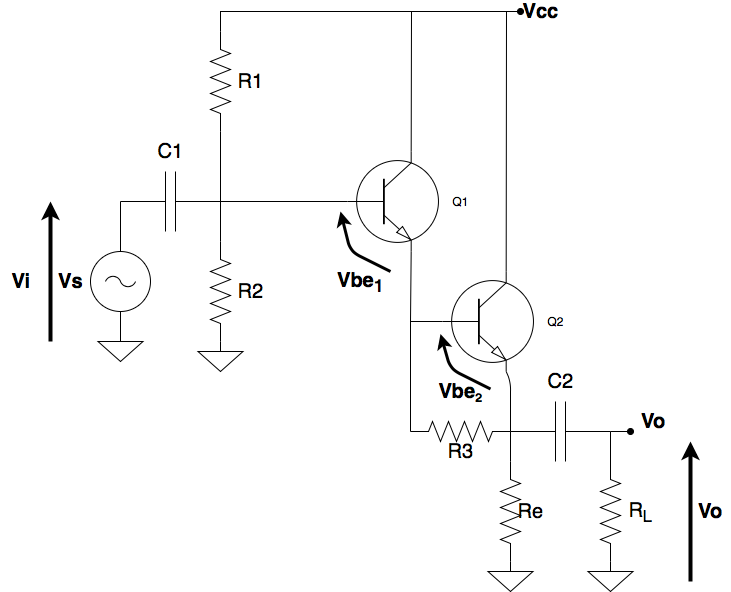
\includegraphics[scale=0.4]{./Imagenes/darlington_tp.png} \\
	\caption{Circuito de estudio en este trabajo, implementando un par Darlington.}
	\label{darlington_tp}
\end{figure}

%\begin{figure}[H]
%	\centering
%	\begin{tabular}{c c}
%		\includegraphics[scale=0.3]{../darlington_ideal.png} &
%		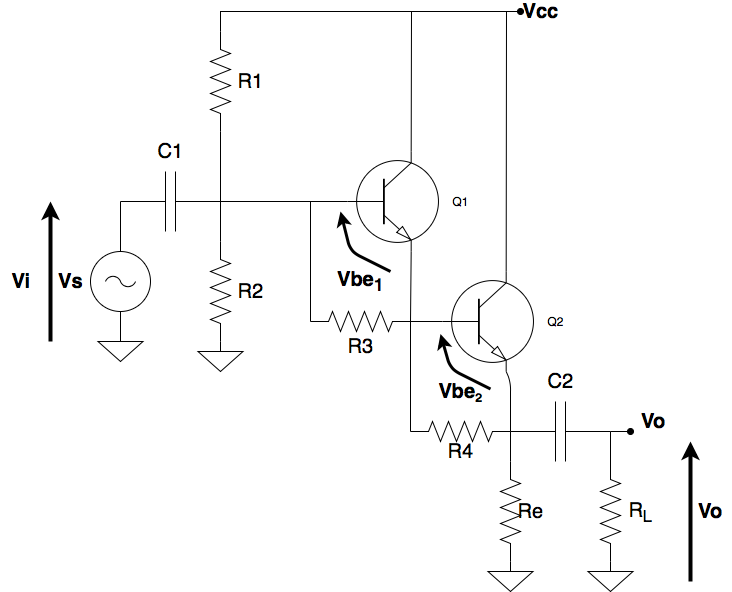
\includegraphics[scale=0.3]{../darlington_tp.png} \\
%	\end{tabular}
%	\caption{}
%	\label{darlington_tp}
%\end{figure}
